\section{算法说明}

\subsection{DQN}
深度 Q 网络(Deep Q-Network,DQN)是一种基于深度学习和强化学习的算法,用于解决离散动作空间的强化学习问题。
\subsubsection{算法流程}
\begin{figure}[H]
    \centering
    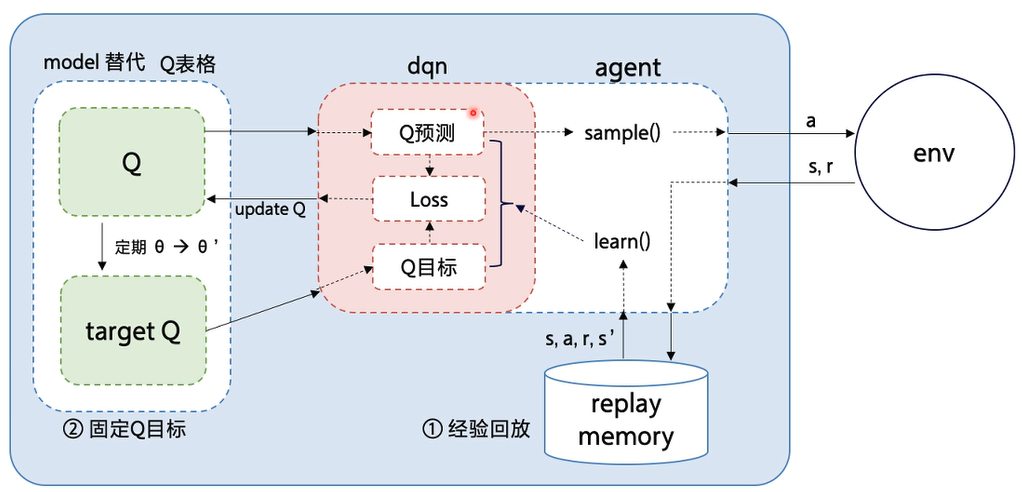
\includegraphics[width=0.8\linewidth]{pic/DQN-process.png}
    \caption{\zihao{-5} DQN算法流程}
    \label{map}
\end{figure}

\subsubsection{算法伪代码}
\begin{figure}[H]
    \centering
    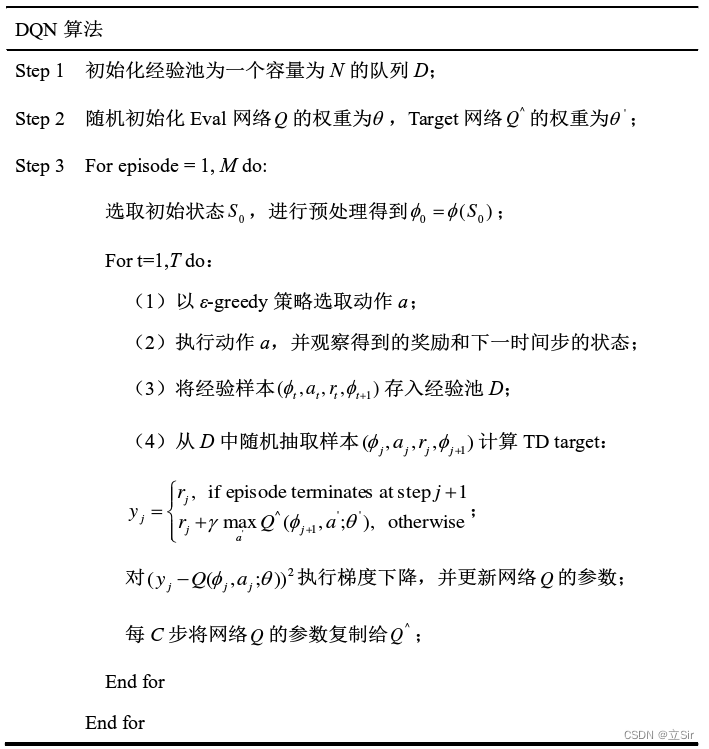
\includegraphics[width=0.8\linewidth]{pic/DQN-code.png}
    \caption{\zihao{-5} DQN算法伪代码}
    \label{map}
\end{figure}

\subsubsection{算法代码}

\begin{enumerate}
    \item 智能体


预测的时候,采用epsilon贪心进行预测。
\begin{lstlisting}[language=Python]
    # epsilon greedy
    if not exploit_flag and np.random.rand(1) < self.epsilon:
        random_action = np.random.rand(batch, self.act_shape)
        random_action = torch.tensor(random_action, dtype=torch.float32).to(self.device)
        random_action = random_action.masked_fill(~legal_act, 0)
        act = random_action.argmax(dim=1).cpu().view(-1, 1).tolist()
    else:
        feature = [
            self.__convert_to_tensor(feature_vec),
            self.__convert_to_tensor(feature_map).view(batch, *self.obs_split[1]),
        ]
        logits, _ = model(feature, state=None)
        logits = logits.masked_fill(~legal_act, float(torch.min(logits)))
        act = logits.argmax(dim=1).cpu().view(-1, 1).tolist()
\end{lstlisting}

学习的时候和预测采用一样的模型计算q\_max,再进一步计算target\_q.
\begin{lstlisting}[language=Python]
    model = getattr(self, "model")
    model.eval()
    with torch.no_grad():
        q, h = model(_batch_feature, state=None)
        q = q.masked_fill(~_batch_obs_legal, float(torch.min(q)))
        q_max = q.max(dim=1).values.detach()

    target_q = rew + self._gamma * q_max * not_done
\end{lstlisting}

\item 模型

模型概览
\begin{figure}[H]
    \centering
    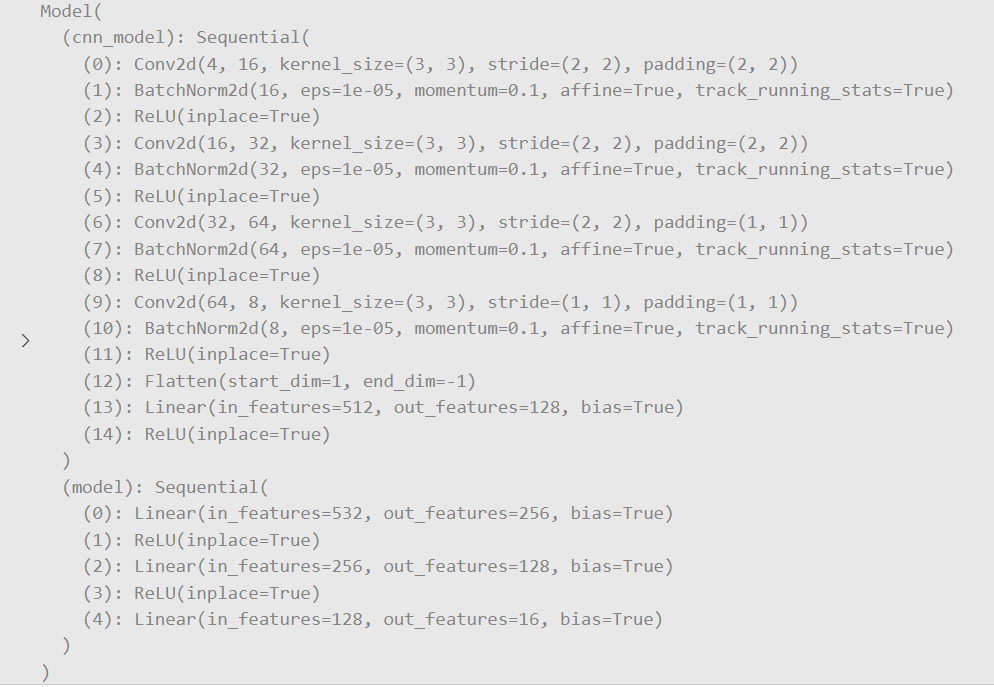
\includegraphics[width=0.8\linewidth]{pic/DQN-model.png}
    \caption{\zihao{-5} DQN算法模型}
    \label{map}
\end{figure}


前向推理

\begin{lstlisting}[language=Python]
# Forward inference
# 前向推理
def forward(self, s, state=None, info=None):
    feature_vec, feature_maps = s[0], s[1]
    feature_maps = self.cnn_model(feature_maps)

    feature_maps = feature_maps.view(feature_maps.shape[0], -1)

    concat_feature = torch.concat([feature_vec, feature_maps], dim=1)

    logits = self.model(concat_feature)
    return logits, state
\end{lstlisting}

 \item 奖励设置

为获得更高的分数,拆解出可能提高或者降低分数的动作,并设置相应的奖励及拼接权重。

\begin{lstlisting}[language=Python]
    """
    Concatenation of rewards: Here are 10 rewards provided,
    students can concatenate as needed, and can also add new rewards themselves
    奖励的拼接: 这里提供了10个奖励, 同学们按需自行拼接, 也可以自行添加新的奖励
    """
    REWARD_CONFIG = {
        "reward_end_dist": "0.1",
        "reward_win": "0.2",
        "reward_buff_dist": "0.001",
        "reward_buff": "0.001",
        "reward_treasure_dists": "0.1",
        "reward_treasure": "0.15",
        "reward_flicker": "0.1",
        "reward_step": "-0.01",
        "reward_bump": "-0.005",
        "reward_memory": "-0.005",
    }

    reward = [
        reward_end_dist * float(REWARD_CONFIG["reward_end_dist"]),
        reward_win * float(REWARD_CONFIG["reward_win"]),
        reward_buff_dist * float(REWARD_CONFIG["reward_buff_dist"]),
        reward_buff * float(REWARD_CONFIG["reward_buff"]),
        reward_treasure_dist * float(REWARD_CONFIG["reward_treasure_dists"]),
        reward_treasure * float(REWARD_CONFIG["reward_treasure"]),
        reward_flicker * float(REWARD_CONFIG["reward_flicker"]),
        reward_step * float(REWARD_CONFIG["reward_step"]),
        reward_bump * float(REWARD_CONFIG["reward_bump"]),
        reward_memory * float(REWARD_CONFIG["reward_memory"]),
    ]
\end{lstlisting}

\end{enumerate}


\subsection{Target-DQN}
\begin{figure}[H]
    \centering
    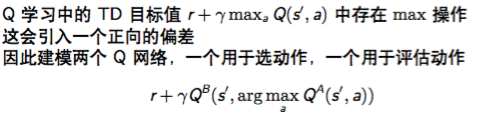
\includegraphics[width=0.8\linewidth]{pic/Double-DQN.png}
    \caption{\zihao{-5} Double-DQN}
    \label{map}
\end{figure}


\subsubsection{算法代码}

\begin{enumerate}
    
\item 智能体

预测的时候,采用epsilon贪心进行预测。这和DQN是一样的。

\begin{lstlisting}[language=Python]
    # epsilon greedy
    if not exploit_flag and np.random.rand(1) < self.epsilon:
        random_action = np.random.rand(batch, self.act_shape)
        random_action = torch.tensor(random_action, dtype=torch.float32).to(self.device)
        random_action = random_action.masked_fill(~legal_act, 0)
        act = random_action.argmax(dim=1).cpu().view(-1, 1).tolist()
    else:
        feature = [
            self.__convert_to_tensor(feature_vec),
            self.__convert_to_tensor(feature_map).view(batch, *self.obs_split[1]),
        ]
        logits, _ = model(feature, state=None)
        logits = logits.masked_fill(~legal_act, float(torch.min(logits)))
        act = logits.argmax(dim=1).cpu().view(-1, 1).tolist()
\end{lstlisting}

学习的时候和预测采用target模型来计算计算q\_max,再进一步计算target\_q.并按照指定步数更新target模型的参数。(和DQN的不同点)
\begin{lstlisting}[language=Python]

    model = getattr(self, "target_model")
    model.eval()
    with torch.no_grad():
        q, h = model(_batch_feature, state=None)
        q = q.masked_fill(~_batch_obs_legal, float(torch.min(q)))
        q_max = q.max(dim=1).values.detach()

    target_q = rew + self._gamma * q_max * not_done
\end{lstlisting}

\begin{lstlisting}[language=Python]

    # Update the target network
    # 更新target网络
    # 按照指定步数更新
    if self.train_step % self.target_update_freq == 0:
        self.update_target_q()
\end{lstlisting}

\item 模型


\begin{figure}[H]
    \centering
    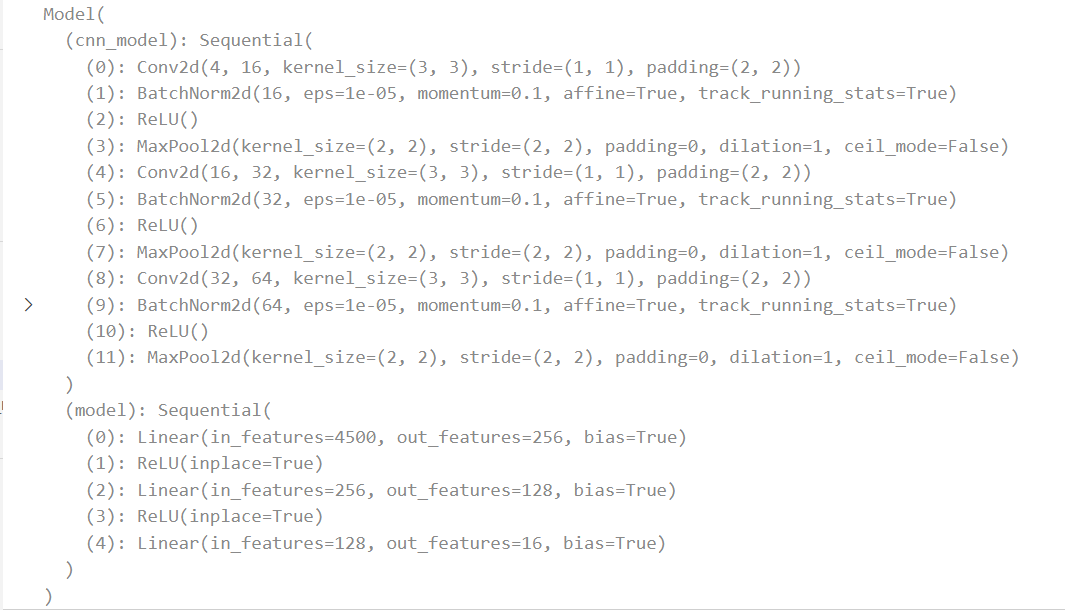
\includegraphics[width=0.8\linewidth]{pic/target-DQN-model.png}
    \caption{\zihao{-5} target-DQN算法模型}
    \label{map}
\end{figure}


\item 前向推理

\begin{lstlisting}[language=Python]
    # Forward inference
    # 前向推理
    def forward(self, s, state=None, info=None):
        feature_vec, feature_maps = s[0], s[1]
        feature_maps = self.cnn_model(feature_maps)

        feature_maps = feature_maps.view(feature_maps.shape[0], -1)

        concat_feature = torch.concat([feature_vec, feature_maps], dim=1)

        logits = self.model(concat_feature)
        return logits, state
\end{lstlisting}

\item 奖励设置

为获得更高的分数,拆解出可能提高或者降低分数的动作,并设置相应的奖励及拼接权重。

\begin{lstlisting}[language=Python]
    """
    Concatenation of rewards: Here are 10 rewards provided,
    students can concatenate as needed, and can also add new rewards themselves
    奖励的拼接: 这里提供了10个奖励, 同学们按需自行拼接, 也可以自行添加新的奖励
    """
    REWARD_CONFIG = {
        "reward_end_dist": "0.1",
        "reward_win": "0.2",
        "reward_buff_dist": "0.001",
        "reward_buff": "0.001",
        "reward_treasure_dists": "0.1",
        "reward_treasure": "0.15",
        "reward_flicker": "0.1",
        "reward_step": "-0.01",
        "reward_bump": "-0.005",
        "reward_memory": "-0.005",
    }

    reward = [
        reward_end_dist * float(REWARD_CONFIG["reward_end_dist"]),
        reward_win * float(REWARD_CONFIG["reward_win"]),
        reward_buff_dist * float(REWARD_CONFIG["reward_buff_dist"]),
        reward_buff * float(REWARD_CONFIG["reward_buff"]),
        reward_treasure_dist * float(REWARD_CONFIG["reward_treasure_dists"]),
        reward_treasure * float(REWARD_CONFIG["reward_treasure"]),
        reward_flicker * float(REWARD_CONFIG["reward_flicker"]),
        reward_step * float(REWARD_CONFIG["reward_step"]),
        reward_bump * float(REWARD_CONFIG["reward_bump"]),
        reward_memory * float(REWARD_CONFIG["reward_memory"]),
    ]
\end{lstlisting}


\end{enumerate}



\subsection{DIY}

\begin{enumerate}
\item DIY1: 修改模型

\begin{lstlisting}[language=Python]
# 前向推理
def forward(self, s, state=None, info=None):
    feature_vec, feature_maps = s[0], s[1]
    feature_maps = self.cnn_model(feature_maps)

    feature_maps = feature_maps.view(feature_maps.shape[0], -1)

    concat_feature = torch.concat([feature_vec, feature_maps], dim=1)

    logits = self.model(concat_feature)

    A = self.fc_layer3_a(logits)
    V = self.fc_layer3_v(logits)
    Q = V + A - A.mean(1).view(-1, 1)  # Q值由V值和A值计算得到

    return Q, state
\end{lstlisting}


\item DIY2: 修改学习函数

\begin{lstlisting}[language=Python]
 
    target_model = getattr(self, "target_model")
    target_model.eval()

    model = getattr(self, "model")
    model.eval()

    with torch.no_grad():
        q, h = model(_batch_feature, state=None)
        max_action = q.max(1)[1].view(-1, 1)
        next_q, next_h = target_model(_batch_feature, state=None)
        next_q = next_q.masked_fill(~_batch_obs_legal, float(torch.min(next_q)))
        q_max = next_q.gather(1, max_action).detach().flatten()
\end{lstlisting}

\end{enumerate}